\chapter{Proposed Methodology}\label{cha:method}
%\begin{preprompt}
%Sketches your basic plan for the system that you will build. If the system is partially built by the midterm delivery deadline, then explain what you have so far along with what you plan to add. In general, the reader should get a good impression of the structure of the complete system that you will eventually deliver for your master's thesis.
%\end{preprompt}

The model we have chosen to implement for this project is the Single Shot Multibox Detector.
The model is relatively small and offers many opportunities to make alterations.
The model is also fairly old by now so it would be natural to update the architecture, e.g.~by changing the backbone model, adding batch normalization, and testing different activation functions.
Newer types of data augmentations have also been proposed and would make for a natural addition.

All object detection systems require the same basic units: a model, data loader, evaluator, and data logger.
Figure~\ref{fig:sys} gives a overview of the system with some of the components broken down further.
Some parts of the system have been prototyped at this stage, while others only have basic functionality.
We will go through the components separately in the next sections

\begin{figure}[htb]
  \centering
  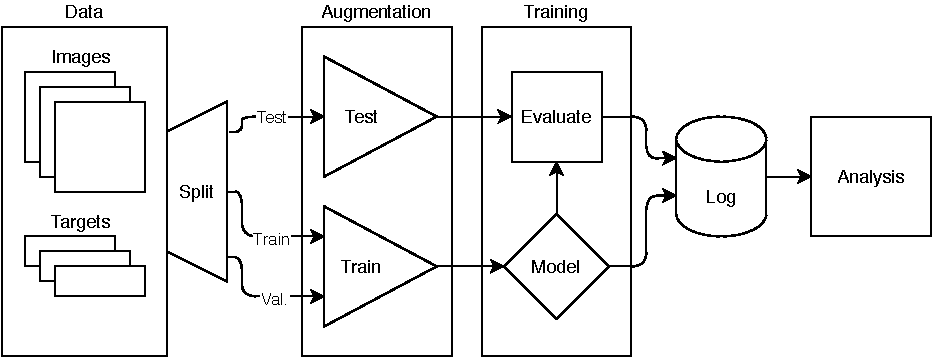
\includegraphics[width=0.7\textwidth]{figs/system.pdf}
  \caption[System overview]{Overview of the basic system components and their interactions.}\label{fig:sys}
\end{figure}

The data loader is responsible for fetching the image files from disk, transforming them to the proper format, and augmenting them.
This system has been developed and is functional.
More types of augmentations can and will be added in the next stage of the project.
The output of the data loader is batches of augmented images and the corresponding labelled bounding boxes.

A prototype of the SSD model has been developed.
The implementation is based on the source code released by the authors.
The main improvements that remain relate to the structure of the system to make it suitable for modification.
It should require no coding to change the backbone model, activation function, batch norm and default box scaling.

The evaluation system has not been developed, only a basic module for visualizing the output of the model.
A completed model would run the model over the testing data and measure the precision, recall, and other relevant performance measures.

%Given that comparable systems are sparse in literature, comparing the system to existing work will give little value or insight.
From the research that has been done in related domains we have seen dif

\section{Sharpness Measure}\label{sec:method-sharpness}
Analyzing how the sharpness of pollen grains affects detection performance requires an objective sharpness measure.
In this section we will detail how sharpness will be measured for the purpose of our analysis.
The measure is based on fourier analysis and its performance has been tested on the training data.

\subsection{Fourier analysis}
Fourier analysis describes the general method of utilizing the fourier transform to analyse the component frequensies present is some signal.
With digital images, we can look at how the brightness changes accross an image following some vector, and use this signal as the basis for our analysis.
An image contains signals in all directions so the fourier transform of an image also encodes this directionality.
Interpreting this value as a signal we can then use the fourier transform to analyse the frequency components of an image, being interpreted as a set of signals.

Using the fourier spectrum to measure sharpness follows from the realization that there is a strong relationship between the sharpness of an image in the spacial domain and the distribution of frequency components in the frequency domain.
Sharp features produce high frequencies while blur smoothes out the changes in brighness, lowering the frequencies.
Figure~\ref{fig:fourier} shows three different pollen grains, captured with progressively more blur.
If we look at their corresponding fourier spectra we can see that, as the percieved blur increases, the amount of high frequency components decrease.
In the figure, the fourier spectra are centered so the lowest frequency component lies in the middle and increases outwards.
The color map is log scaled so that the higher frequencies become visible.

\begin{figure}[htbp]
  \centering
  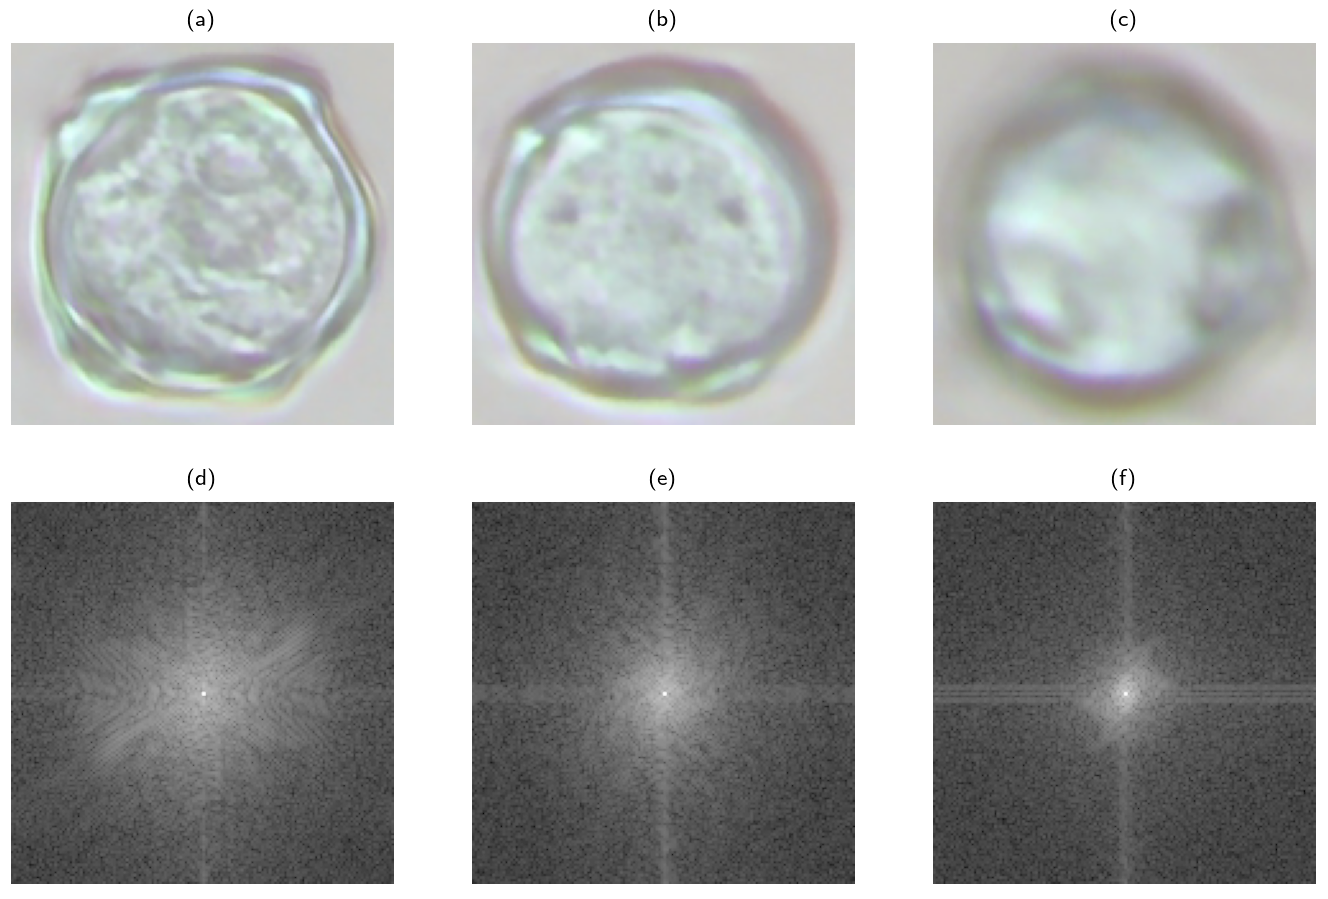
\includegraphics[width=0.8\textwidth]{figs/fourier.png}
  \caption[Fourier spectrum]{Pollen grains and their coresponding centered fourier spectrum.}\label{fig:fourier}
\end{figure}

\subsection{Measuring sharpness}
We must then decide how to encode this change in frequency distridution as a scalar sharpness measure.
\citeauthor{de2013image} propose a simple method which counts the number of components in the fourier spectrum having a value above a certain threshold.
The operation is described in Equation (\ref{eq:sharp}).


\begin{equation}\label{eq:sharp}
  \begin{split}
    \mathbf{X} = \mathcal{F}(a),\quad a\in \mathbb{Z}^{M\times N}\\
    T_H = \sum_{x\in\mathbf{X}}[x\ge\mu],\quad \mu=\frac{\max \mathbf{X^{\mathrm{abs}}}}{1000}\\
    S = \dfrac{T_H}{M\times N}
  \end{split}
\end{equation}

Here \(\mathcal{F}\) is the dicrete the fourier fransform, operationg on a input image \(a\), and \(\mathbf{X}\) only contains the magnitude of the fourier transform.
The scaling factor of the threshold value, \(\mu \), was found to produce good results on our data, without modification.

Validating the sharpness measure is an important task.
The weight of any argument made based on analysis using this measure is predicated on its soundness.
There are many different approches to this, we have chosen to compare the objective measure with subjective measurements of percieved sharpness on a subset of the training data.

\subsection{Evaluating the sharpness measure}

A small subset of the dataset is chosen at random and a human assessment is performed to determine the sharpness of every labeled pollen grain.
This can then be used to score the different sharpness measures.
Determining the sharpness of a pollen grain with high fidelity was found to be very subjective and non-reproducible, so a simple classification was instead performed.
Images are separated into three classes.
Figure~\ref{fig:fourier} gives examples of the three classes with image (a) being the sharpest (class 3) and (c) being the blurriest (class 1).
In total 389 grains where evaluated, the distribution of their classes is given in Table~\ref{tab:sharpness}

\begin{table}[htb]
  \caption[Sharpness dataset distribution]{Distribution of classes accross the sharpness validation dataset.}\label{tab:sharpness}
  \centering 
  \begin{tabular}{lr} \toprule
    Sharpness & Frequency \\ \midrule
    1 --- blurred & 123 \\
    2 & 105 \\
    3 --- sharp & 125 \\ \bottomrule
  \end{tabular}
\end{table}

Looking at Figure~\ref{fig:sharpness} we can see a clear correlation between the mean of the distribution, and the percieved sharpness.
The overlap is to be expected, given the mapping from a continuous predictor onto a categorical label.
To further evaluate the performance of the sharpness measure, we construct a very simple statistical model, in the form of a decision tree, and test its ability to differentiate between the classes.
The model achived a test accuracy of 84.1\%.

\begin{figure}[htbp]
  \centering
  \begin{subfigure}[t]{0.49\textwidth}
    \centering
    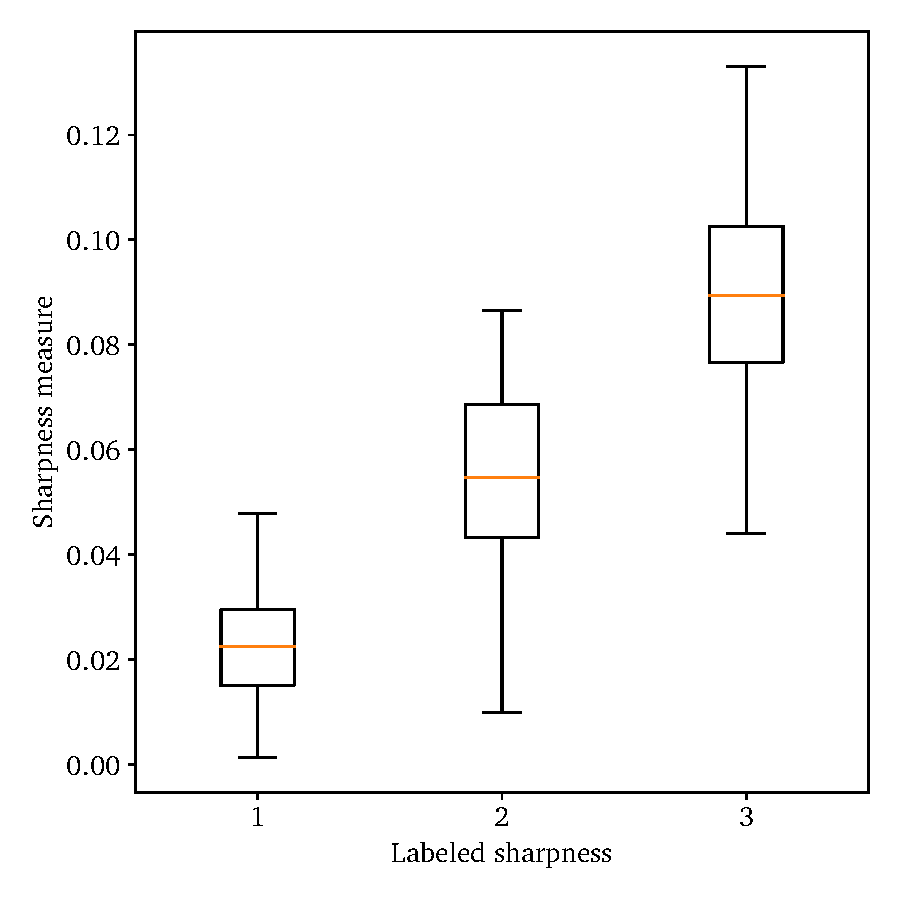
\includegraphics[width=\textwidth]{figs/box.pdf}
    \caption{Box plot}\label{fig:sharpness-box}
\end{subfigure}%
\hfill
\begin{subfigure}[t]{0.48\textwidth}
  \centering
  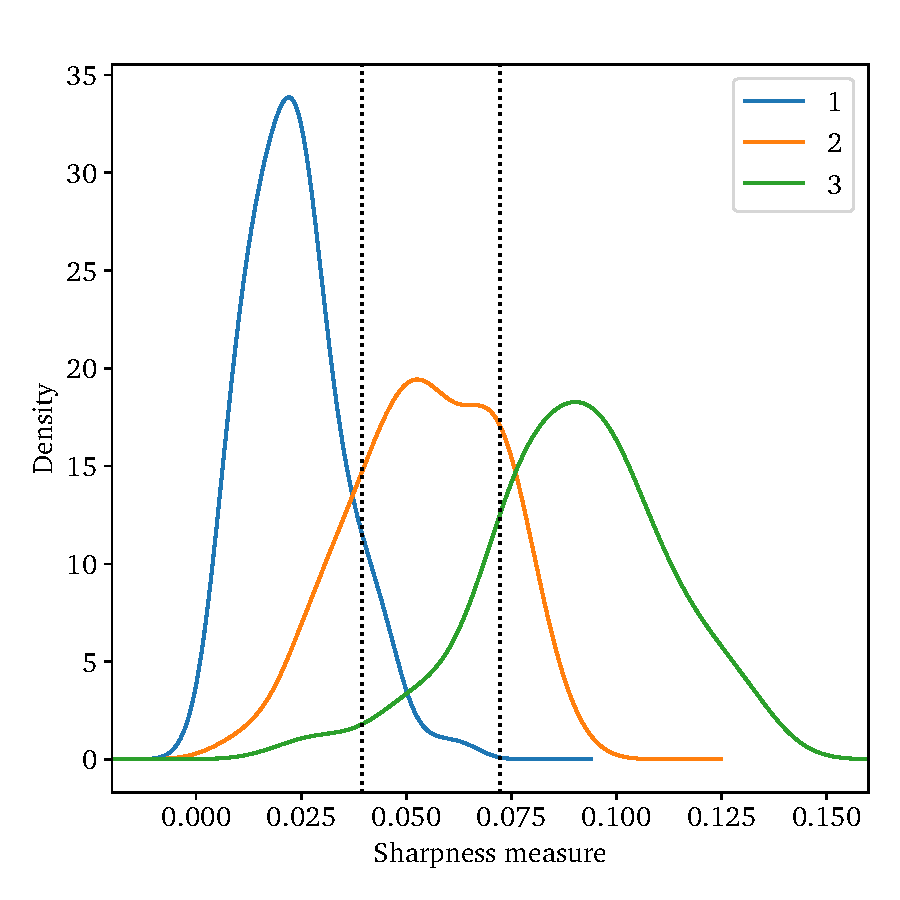
\includegraphics[width=\textwidth]{figs/qden.pdf}
  \caption{Density plot}\label{fig:sharpness-qden}
\end{subfigure}
  \caption[Sharpness measure seperability]{The sharpness measure grouped by class label. Although there is an overlap between ajacent classes, there is a clear seperation between the IQR of measured sharpness in (a). The correlation between percieved and measured sharpness is also clear.}\label{fig:sharpness}
\end{figure}
